\subsection{Counterexamples improve screening before they repay acquisition}

The separately frozen development probe executes the DOCX's challenge process. Three seeded defective creator artifacts produce substantiated objections, corrected outputs and retained regression cases. Two objections come from the bounded challenger; the locked-bound case is a review-specified counterexample. A fourth, deliberately false objection claims that overlapping jobs necessarily violate a pooled crew constraint. The adjudicator refutes it because concurrent demand equals available capacity. The correct result is retained.

The probe then compares seven prespecified candidate variants on 14 new diagnostic cases, with no protected confirmation inputs. Without early assets, the unchanged final checker uses 70 calls and 105,994 reference units. Screening the retained counterexamples first reduces these to 37 calls and 53,721 units. Acquisition and retention cost 41,785 units, while retrieval adds 27,177. The first batch therefore costs \textbf{122,683 units}, a \textbf{16,689-unit loss}. The conventional regression suite given the same assets produces exactly the same checks, costs and decisions.

All arms retain one valid candidate and reject six flawed variants. Final correctness does not improve. The useful change is \emph{earlier} exposure of particular defects; the valid candidate pays additional screening overhead. Repeating the identical batch would save 25,096 recurring units after retrieval, giving a modeled two-batch acquisition payback. That calculation assumes the same future defect mix and does not establish observed demand, a population effect or profit.

This probe's frozen tariff charges one reference unit per retained or retrieved byte, unlike the main study's 64-byte envelope/checkpoint blocks. Its payback boundary is conditional on that declared model. The two unit systems are not added together or treated as physical CPU costs.

\begin{figure}[ht]\centering
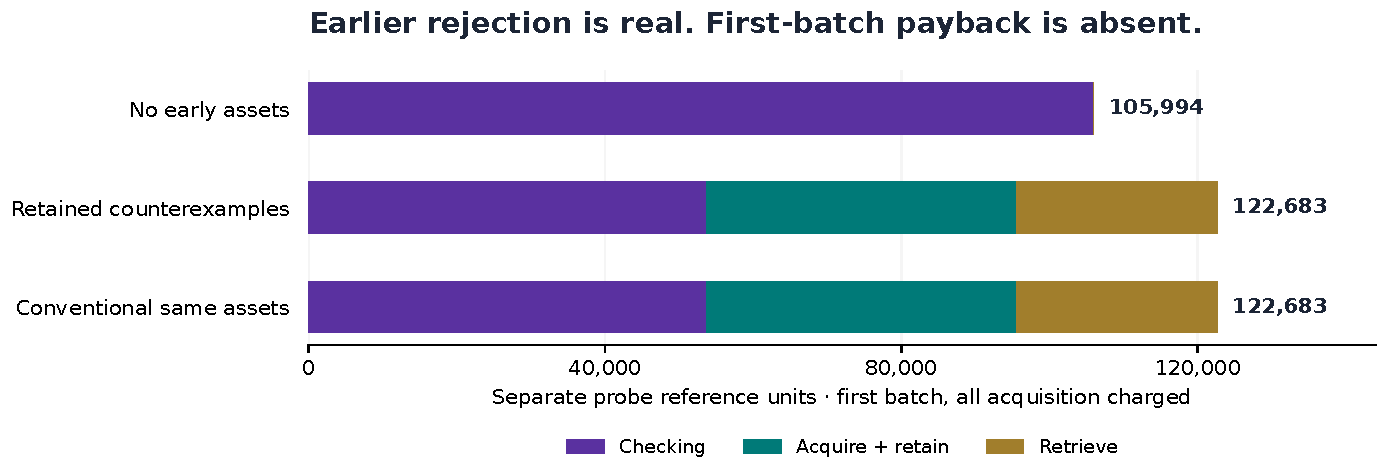
\includegraphics[width=\linewidth]{figures/regression-costs.pdf}
\caption{A verified counterexample is an asset with a carrying cost. Earlier rejection cuts checking work, but acquisition and retrieval reverse the first-batch saving. The conventional asset control is exactly equal. These are the separate development probe's reference units, not pooled main-study work units.}\label{fig:regression-costs}
\end{figure}

The raw challenge evidence, independent adjudications, revisions, regression assets, prospective probe protocol and frozen source identities are included under \artifact{review/}. The probe's seven deliberately seeded variants are not a random sample of production defects; no statistical population claim is made. Evaluator source and the final acceptance predicate remain unchanged throughout.
